\chapter{Physics at lepton colliders}
\label{Lepton_Physics}
\begin{chapterabstract}
The physics at particle colliders, where two particle beams are brought into collision, is the physics of atoms and quanta, of nuclei and partons, of particles that build up everything we know, but also of new particles, physics beyond our current knowledge.
After a brief introduction of the Standard Model, a theory describing the elementary particles and the fundamental forces, the physics processes at a lepton collider will be explained in more detail.
\end{chapterabstract}
\newline

Particle physics extends back to the ancient Greek times, when the idea was developed that matter is made of ``indivisible'' (\'atomos, Greek) parts.
Atoms are, in fact, not indivisible at all.
When the electron was experimentally discovered in 1897 by J.J. Thomson, it was proposed that these particles must be a component of every atom.~\cite[p. 13ff]{Griffiths}
This sparked the interest of many physicists in the early \nth{20} century to perform experiments probing atoms.
One of them was Ernest Rutherford, who fired alpha particles\footnote{An alpha particle is the nuclei of a Helium atom. Ernest Rutherford obtained them from decays of uranium and other radioactive elements.} through a thin gold foil, and thereby found that atoms are mostly empty with a positively charged nucleus that is only a fraction of the size of the atom itself.
\todo{It would be cool if you could find a reference to the Gold Foil experiment}
This discovery was a crucial step towards the modern atomic model.\\
Closer to our current understanding of the atomic model is the Bohr model, developed by Niels Bohr in 1914.~\cite[p. 15]{Griffiths}
It asserts that electrons orbit the positively charged nucleus on stable shells with distinct radii.
The shells correspond to discrete energies, such that an electron switching from one shell to a shell with a larger radius would have to absorb energy, or emit energy respectively.
This energy quantum is absorbed or emitted in the form of light, or more precisely, in the form of a photon.
Nowadays, it is known that the electrons do not orbit the nucleus on discrete shells but rather in orbital zones, where the electron has a higher probability to be observed.\\
In order for an atom to have a neutral charge, the number of electrons in the atomic shells have to be balanced by an equal amount of positive charge in the nucleus.
That nuclei of different atoms are built from the hydrogen nucleus was already proven by Rutherford.
He thereby discovered the proton, and explained that the positive charge of the nucleus is the summed up charges of the protons inside the nucleus.\\
In 1932, it was found that atoms can not only consist of electrons and protons.~\cite[p. 15]{Griffiths}
The mass measurements of various isotopes showed that their masses differ by concrete amounts.
The explanation was that the nucleus must consists of protons and particles with a similar mass but a neutral charge, the neutrons.
\todo{You can reference Chadwick here for discovering the neutron if you want}
Isotopes are therefore atoms of the same element with the same number of electrons and protons, but with a different amount of neutrons.\\
Over the years, the development of particle accelerators that can accelerate particles to higher and higher energies allowed to probe even the constituents of the atom.
This showed that the end has not been reached yet, that protons and neutrons are not elementary but composite particles.
Their partons, the so-called quarks, are part of the current theory of all elementary particles and the fundamental forces they interact with, the Standard Model.
\section{The Standard Model}
\label{StandardModel}
The Standard Model (SM) was developed and formulated around the 1960s and 1970s, when the theories of the electromagnetic and the strong interaction, namely quantum electrodynamics (QED)~\cite{QED,QED2,QED3} and quantum chromodynamics (QCD)~\cite{QCD,QCD2}, were combined into one mathematical model that explains how the elementary particles interact with each other via the fundamental forces of the universe.~\cite[p. 3]{Griffiths}
Since then, high-energy particle physics experiments could verify the SM predictions so well, that it has proven itself to currently be the best theoretical model of all subatomic particles physics that we know of.\\
The SM differs between two classes of the fundamental particles: 
the particles that make up all matter are called \textit{fermions}, whilst the force mediators, through which the fermions can interact, are called \textit{gauge bosons}.
\begin{figure}[h]
\centering
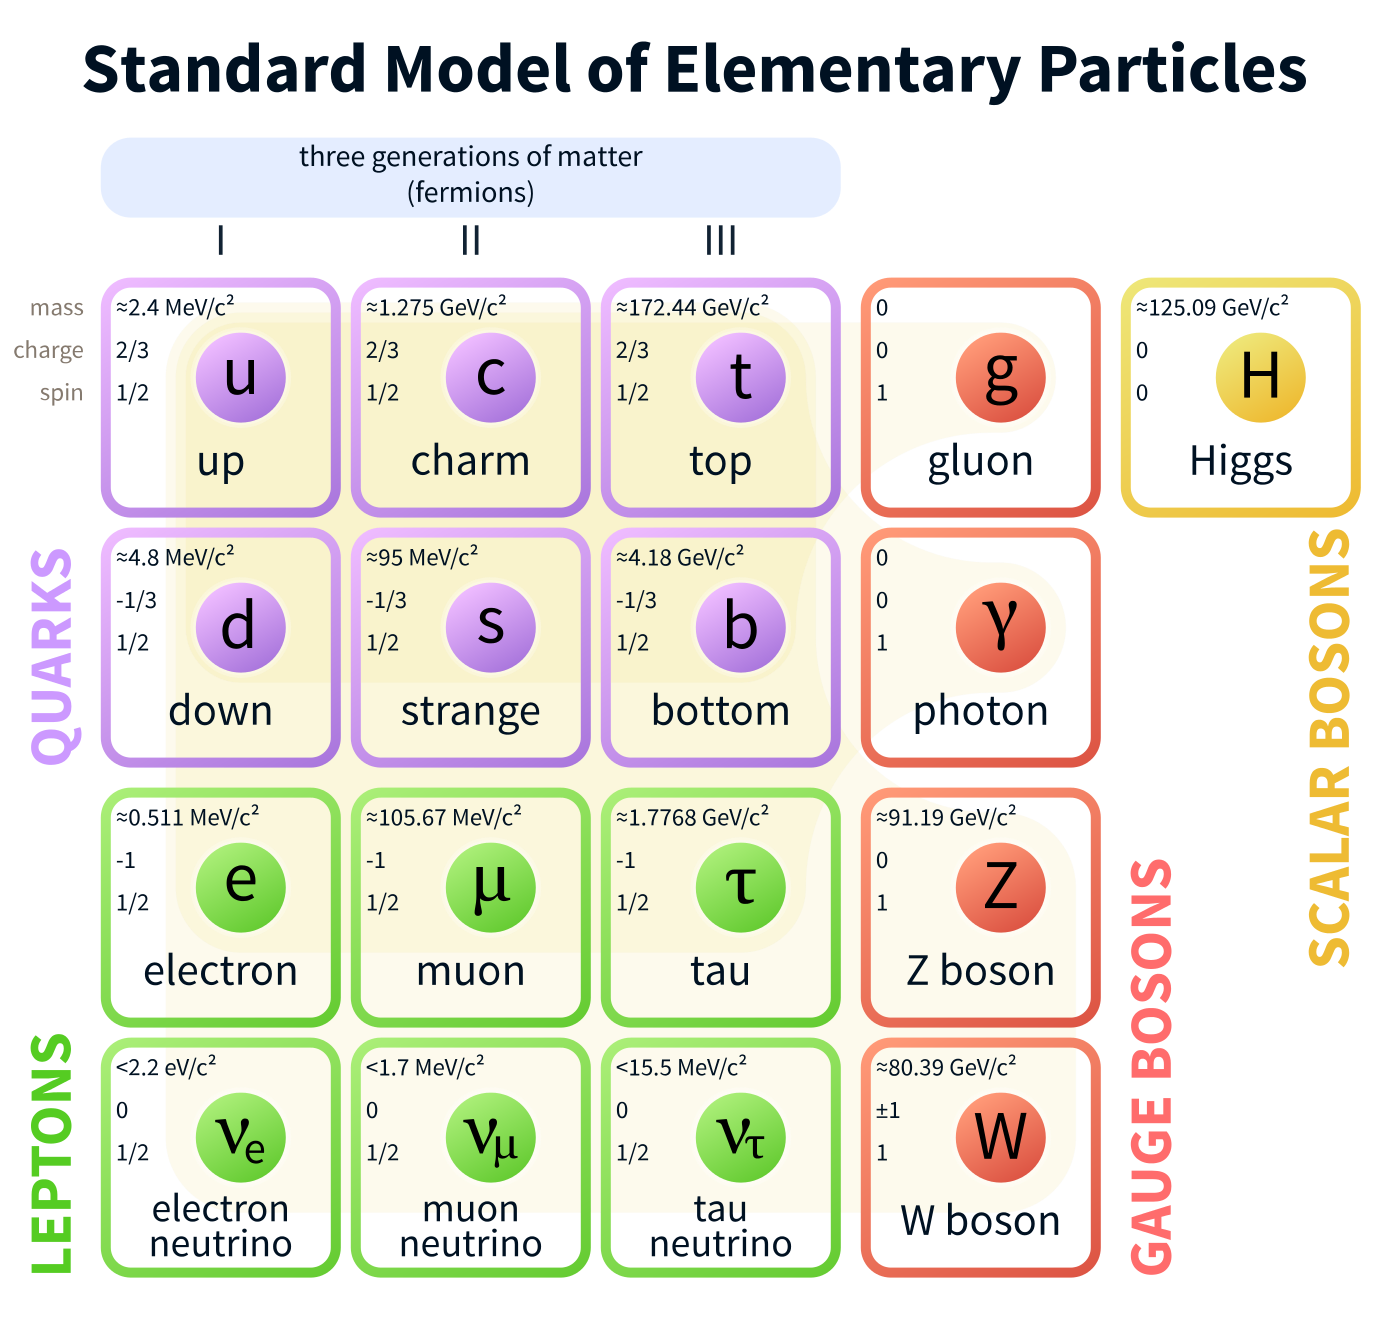
\includegraphics[width=0.53\textwidth]{Figures/Standard_Model_of_Elementary_Particles.png}
\caption[Standard Model]{The Standard Model describes all elementary particles, the twelve fermions in their three generations and the four gauge bosons, as well as the Higgs boson.
The shadows indicate possible interactions between the fermions and gauge bosons.~\cite{SM}}
\label{fig:SM}
\end{figure}
\todo{The shadows are very difficult to see. If you want you can use the picture from my thesis}

\paragraph{Fermions}
Fermions are particles with a spin quantum number of $s = 1/2$. 
The spin is the particle's rotation about its central axis, and has a direction and a specific amplitude.
\todo{The particles don't actually have a spin, there is no central axis for something that is point like. It is just a quantum number that behaves similar to how spin behaves on large objects}
The amplitude can be calculated as $\frac{h}{2\pi}\sqrt{s(s+1)}$, with $h$ being the Planck constant.~\cite[p. 121]{Griffiths}
All fermions have a specific set of quantum numbers, so that by giving the electric charge, the spin, and the flavor, all fermions can be identified precisely.
Table~\ref{tab:Fermions} lists all Standard Model fermions with their quantum numbers.
\begin{table}
\caption[Quantum numbers of the Standard Model fermions]{Quantum numbers of the Standard Model fermions. The table lists the values for the electric charge $q$, and the spin $s$ for all fermions, as well as the lepton number $L$ of the leptons and the quark flavor of the quarks. Their respective antiparticles are highlighted by the shaded background.~\cite[cf. p. 49]{Griffiths}}
\label{tab:Fermions}
\centering
\begin{tabularx}{\textwidth}{c|c|rrrrr|@{\hskip 0.03in}|c|rrrrrrrr}
\hline\hline
& Leptons & $q$ & $s$ & $L_e$ & $L_{\mu}$ & $L_{\tau}$ & Quarks & $q$ & $s$ & $U$ & $D$ & $C$ & $S$ & $T$ & $B$\\
\hline
& e\textsuperscript{--} & --1 & 1/2 & +1 & 0 & 0 & u & +2/3 & 1/2 & +1 & 0 & 0 & 0 & 0 & 0\\
\rowcolor{Gray}
\cellcolor{white}& e\textsuperscript{+} & +1 & 1/2 & --1 & 0 & 0 & $\bar{\rm{u}}$ & --2/3 & 1/2 & --1 & 0 & 0 & 0 & 0 & 0\\
& $\upnu$\textsubscript{e} & 0 & 1/2 & +1 & 0 & 0 & d & --1/3 & 1/2 & 0 & --1 & 0 & 0 & 0 & 0\\
\rowcolor{Gray}
\multirow{-4}{*}{\rotatebox[origin=c]{90}{\parbox[c]{1.9cm}{\cellcolor{white}\centering First generation}}} &$\bar\upnu$\textsubscript{e} & 0 & 1/2 & --1 & 0 & 0 & $\bar{\rm{d}}$ & +1/3 & 1/2 & 0 & +1 & 0 & 0 & 0 & 0\\
\hline
& $\upmu$\textsuperscript{--} & --1 & 1/2 & 0 & +1 & 0 & c & +2/3 & 1/2 & 0 & 0 & +1 & 0 & 0 & 0\\
\rowcolor{Gray}
\cellcolor{white}&$\upmu$\textsuperscript{+} & +1 & 1/2 & 0 & --1 & 0 & $\bar{\rm{c}}$ & --2/3 & 1/2 & 0 & 0 & --1 & 0 & 0 & 0\\
& $\upnu$\textsubscript{$\upmu$} & 0 & 1/2 & 0 & +1 & 0 & s & --1/3 & 1/2 & 0 & 0 & 0 & --1 & 0 & 0\\
\rowcolor{Gray}
\multirow{-4}{*}{\rotatebox[origin=c]{90}{\parbox[c]{1.9cm}{\cellcolor{white}\centering Second generation}}}& $\bar\upnu$\textsubscript{$\upmu$} & 0 & 1/2 & 0 & --1 & 0  & $\bar{\rm{s}}$ & +1/3 & 1/2 & 0 & 0 & 0 & +1 & 0 & 0\\
\hline
& $\uptau$\textsuperscript{--} & --1 & 1/2 & 0 & 0 & +1 & t & +2/3 & 1/2 & 0 & 0 & 0 & 0 & +1 & 0\\
\rowcolor{Gray}
\cellcolor{white}& $\uptau$\textsuperscript{+} & +1 & 1/2 & 0 & 0 & --1 & $\bar{\rm{t}}$ & --2/3 & 1/2 & 0 & 0 & 0 & 0 & --1 & 0\\
& $\upnu$\textsubscript{$\uptau$} & 0 & 1/2 & 0 & 0 & +1 & b & --1/3 & 1/2 & 0 & 0 & 0 & 0 & 0 & --1\\
\rowcolor{Gray}
\multirow{-4}{*}{\rotatebox[origin=c]{90}{\parbox[c]{1.9cm}{\cellcolor{white}\centering Third generation}}}& $\bar\upnu$\textsubscript{$\uptau$} & 0 & 1/2 & 0 & 0 & --1 & $\bar{\rm{b}}$ & +1/3 & 1/2 & 0 & 0 & 0 & 0 & 0 & +1\\
\hline\hline
\end{tabularx}
\end{table}
\todo{Fix the incorrect plus and minus for quarks}
\todo{Remove the double minus to make it visible in all PDF viewers}
Fermions are further categorized as \textit{leptons} and \textit{quarks}, as well as in three generations, which can be seen in Figure~\ref{fig:SM}.
Among the leptons are the electron and its heavier brothers, the muon and the tau.
In their respective generation, each of them has a neutrino, respectively named the electron-neutrino, muon-neutrino, and tau-neutrino, and they are electrically neutral particles.\\
Since the SM does in general not remark the corresponding antiparticles, there are actually not only six leptons but twelve.
\todo{I would reword this into maybe 2 or 3 sentences, referring to the fat that every particle has an antiparticle, that all of their quantum numbers are opposite, they are excluded from discussion because they don't add anythihng in terms of physics...}
The only difference between particles and antiparticles is the sign of their internal quantum numbers:
The electron's antiparticle is the positron, which has the same mass and spin as the electron, but has a positive charge of +1, and a negative lepton number $L_e$ of -1.
The antiparticles of the muon ($\upmu$\textsuperscript{-}) and the tau ($\uptau$\textsuperscript{-}) hence are $\upmu$\textsuperscript{+} and $\uptau$\textsuperscript{+}, respectively.
As neutrinos on the other hand have no electric charge, they can only be distinguished from their respective antineutrino by their lepton number and their helicity.
The helicity describes the state of the particle's spin direction in comparison to the particle's momentum.
When the spin direction and the momentum are parallel, the particle is called right-handed.
It is called left-handed, when they are antiparallel.
In the SM, neutrinos are always left-handed, whilst antineutrinos are right-handed.\\
Every generation of quarks consists of one up- and one down-type quark, where the up-type quarks have an electric charge of 2/3, whilst down-type quarks have a charge of --1/3.
\todo{remove the --}
However, they do not only carry the electric charge, but also the so-called color charge.
Every quark has one of three colors (red, green, and blue), every antiquark has one of three anti-colors (anti-red, anti-green, and anti-blue).
Thus, there are overall 36 different quarks and antiquarks.
Due to the law of confinement, there can only be color-neutral particles.
\todo{What does color neutral mean?}
Quarks are therefore not free, but hadronize and form a bound state together with other quarks.
These bound quark states, called hadrons, consist of either two, three, or five quarks.
A particle with a quark of a specific color and an antiquark of the corresponding anti-color is called a meson.
A baryon, which is a particle with three quarks, can only be color-neutral when it carries three quarks with three different colors (or anti-colors), so red--green--blue or anti-red--anti-green--anti-blue, any other combination is not possible.
\todo{ remove the --}
Finally, the penta-quarks are bound states of five quarks, where three of them form a color triplet like a baryon, and the remaining two form a color-anticolor pair like a meson.\\
In everyday nature, the only observable hadrons are the protons and neutrons due to their constituents.
They are baryons, hence are built from three quarks:
protons contain two up-quarks and one down-quark, giving the proton its positive electric charge of +1.
Neutrons on the other hand are formed by one up-quark and two down-quarks, resulting in an electrically neutral particle. 
As the up-quark is the lightest quark, it is stable and does not decay.
All other quarks decay after certain lifetimes into another quark with smaller mass.
That is the reason why all hadrons that are produced artificially in a high-energy particle collider are unstable.
Since the down-quark is the second lightest quark, it can decay into the up-quark, giving reason to the spontaneous decay of free neutrons into protons when one of the down-quark decays.
The proton is the lightest existing hadron, and does not decay further.
\todo{Why can I proton not decay to something like a lighter meson?}
Together, the protons and neutrons construct the nuclei of every atom of every element.
%The masses of the quarks increases towards higher generations.

\paragraph{Bosons}
The \textit{gauge bosons} described in the SM are the force mediators of the fundamental forces of nature:
the electromagnetic, the weak, and the strong force.
Gravity is the only fundamental force that is not represented by the SM.
On the scale of particle physics, it is by far the weakest force, as can be seen from Table~\ref{tab:Forces}.
\begin{table}
\caption[Fundamental forces]{The fundamental forces and their mediators.~\cite[cf. p. 59]{Griffiths}
The strength of a force is dependent on various external factors.
Therefore, the listed values are a rough guideline of the orders of magnitude of difference between the effective strengths of the forces.}
\label{tab:Forces}
\centering
\begin{tabularx}{0.45\textwidth}{l|ll}
\hline\hline
Force & Strength & Mediators\\
\hline
Strong & \num{10} & Gluons\\
Electromagnetic & \num{e-2} & Photons\\
Weak & \num{e-13} & W, Z\\
Gravitational & \num{e-42} & Gravitons\\
\hline\hline
\end{tabularx}
\end{table}
\\The fermions explained in the paragraph above are subject to these fundamental forces, and can interact with each other by exchanging the force mediators.
The mediating particles are gauge bosons, which are particles with a spin of +1.\\
\begin{minipage}{0.55\textwidth}
The \textit{photon} is a massless, electrically neutral particle mediating the electromagnetic (EM) force between electrically charged particles only.
Since the EM interaction, which is pictured in Figure~\ref{fig:Feynman:EM}, does not change the flavor of the particle, the photon therefore couples to all charged SM particles and their antiparticles, so that the electric charge is conserved in this interaction.
%The mathematically formulated theory of all interactions involving the electromagnetic force in the context of particle physics is given in the theory of quantum electrodynamics (QED).
%Although its reach is in principle not limited by its mass, the effective range of the electromagnetic force is dependent on its potential, which scales with $1/r$. \todo{Potential of electroweak interaction}
\end{minipage} \hfill
\begin{minipage}{0.4\textwidth}
\centering
\begin{figure}[H]\centering
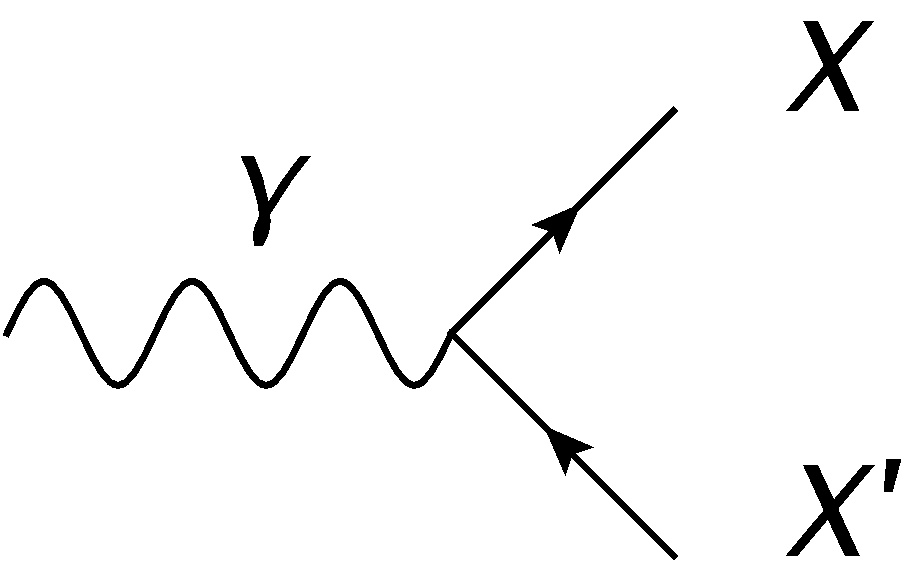
\includegraphics[width=0.5\textwidth]{Feynman_diagrams/Jaxo_EM.png}
\caption{SM Feynman diagram of the EM interaction}
\label{fig:Feynman:EM} 
\end{figure}
\end{minipage}

\begin{minipage}{0.55\textwidth}
\textit{Gluons} are massless particles as well.
They carry the strong force, and like the quarks they are also color-charged, because of which they cannot occur in isolation.
Due to their color-charge, gluons only couple to quarks or to themselves.
The latter is called gluon self-coupling.\\
The gluons mediating the strong force bind the quarks together in all hadrons.
Since the proton is the only stable hadron, it used for high-energy particle physics experiments to probe the proton and investigate its constituents.
This probing is called ``deep inelastic scattering'', where an electron for instance is brought into collision with a proton.
The electron penetrates the proton and scatters on one parton.
By observing such processes, the distribution of the partons inside the proton can be determined, and summarized as the ``parton distribution functions''.
Free partons, such as the remaining constituents of the proton, hadronize due to the color confinement, and form clusters of hadrons, so-called ``jets''.
  \todo{You like to say so-called a lot}

\end{minipage} \hfill
\begin{minipage}{0.4\textwidth}
\centering
\begin{figure}[H]\centering
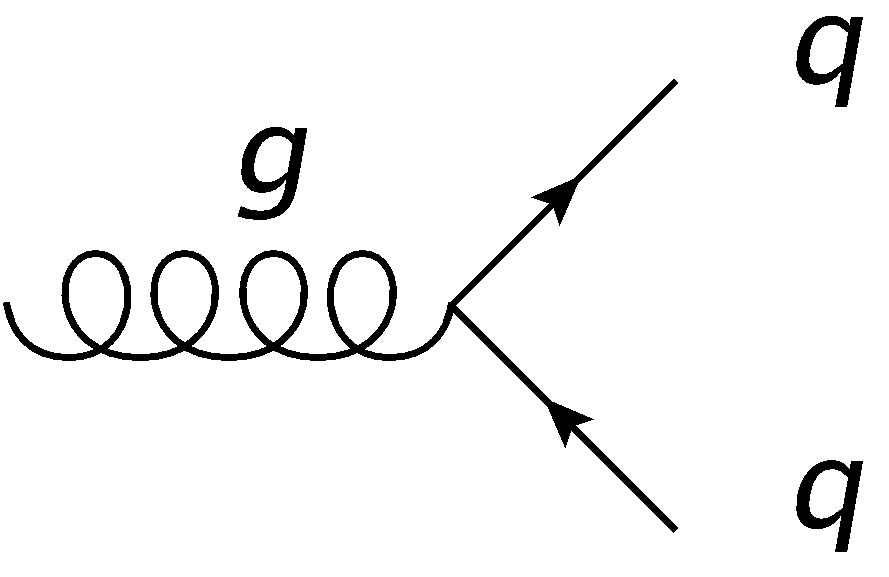
\includegraphics[width=0.5\textwidth]{Feynman_diagrams/Jaxo_strong.png}
\caption{SM Feynman diagram of the strong interaction}
\label{fig:Feynman:strong} 
\end{figure}
\end{minipage}

\begin{minipage}{0.55\textwidth}
\textit{W$^\pm$ and Z$^0$ bosons} on the other hand are massive particles, which are responsible for the weak force.
All fermions can interact via the weak force, also the neutrinos which cannot interact via any other force.
Weak interactions differ between particles of certain handedness, and can therefore only be undertaken by left-handed particles and right-handed antiparticles.
Due to the electric charge of the W$^\pm$ boson, its exchange involves a transfer of electric charge, and is therefore called ``charged current''.
The exchange of the neutral Z boson on the other hand is called ``neutral current''.\\
Similar to the electromagnetic interaction via a photon, the electric charge has to be conserved in the neutral current interaction as well, which is shown in Figure~\ref{fig:Feynman:weak} (a).
Therefore, the flavor of the fermions involved in this first-order interaction does not change, since only particle--antiparticle pairs are taking part.
  \todo{Double minus again}
Interactions involving a W boson on the other hand can either be between a lepton and a neutrino (Figure~\ref{fig:Feynman:weak} (b)), or between an up- and a down-type quark (Figure~\ref{fig:Feynman:weak} (c)). 
In both cases, the flavor of the particles can change, so that interactions between all generations are possible.
\end{minipage} \hfill
\begin{minipage}{0.4\textwidth}
\centering
\begin{figure}[H]
\centering
\begin{subfigure}[b]{\textwidth}\centering
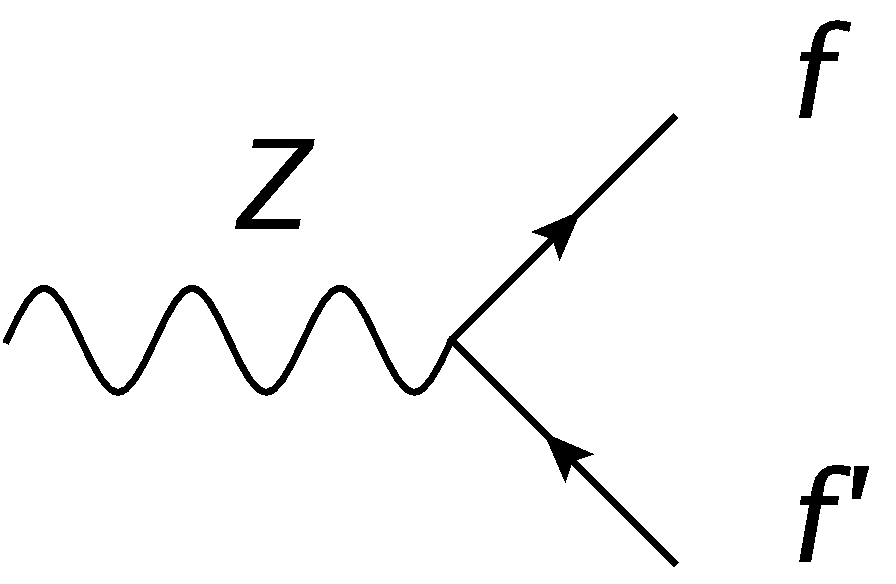
\includegraphics[width=0.5\textwidth]{Feynman_diagrams/Jaxo_weak_Z.png}
\caption{Z boson couples to any SM fermion and its antiparticle}
\end{subfigure}\\
\begin{subfigure}[t]{0.48\textwidth}\centering
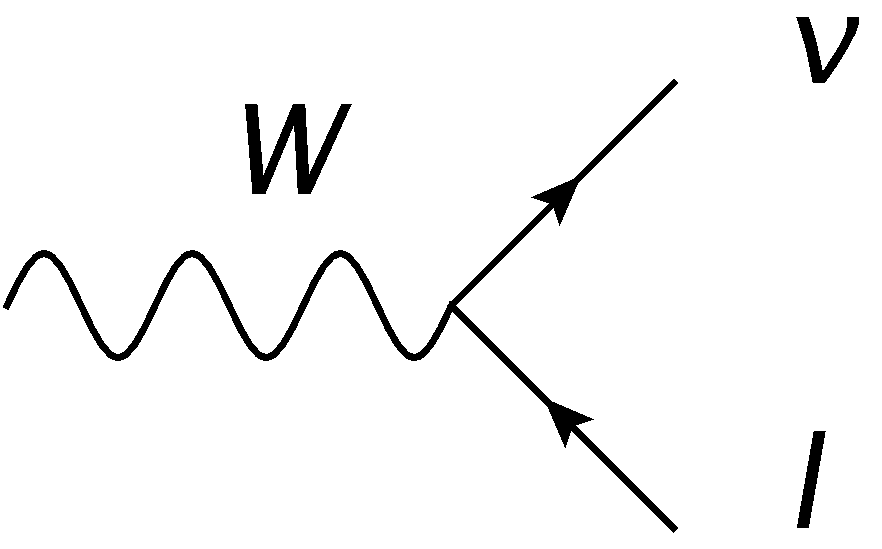
\includegraphics[width=\textwidth]{Feynman_diagrams/Jaxo_weak_W_leptons.png}
\caption{W boson couples to any SM lepton and its corresponding neutrino}
\end{subfigure}\hfill
\begin{subfigure}[t]{0.48\textwidth}\centering
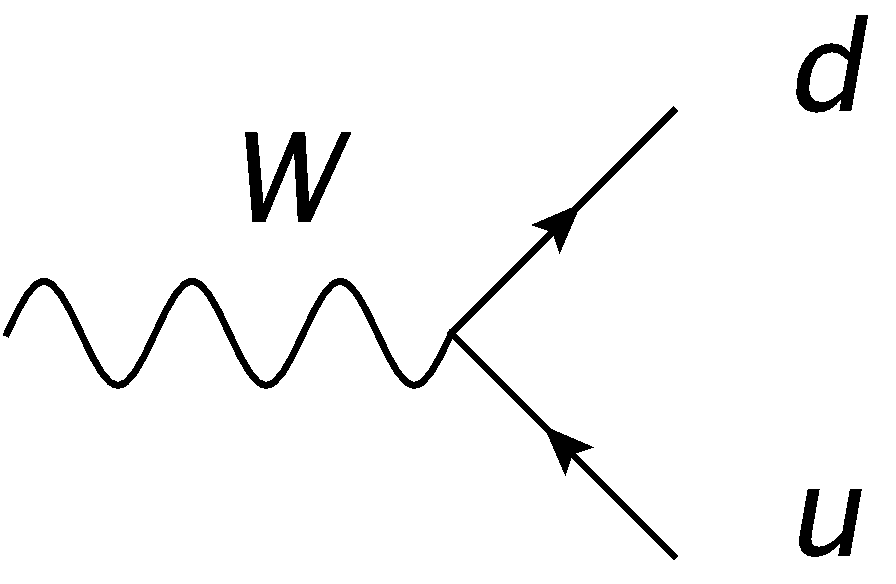
\includegraphics[width=\textwidth]{Feynman_diagrams/Jaxo_weak_W_quarks.png}
\caption{W boson couples to any SM up-type and down-type quark}
\end{subfigure}
\caption{SM Feynman diagram of the weak interactions}
\label{fig:Feynman:weak} 
\end{figure}
\end{minipage}

In contrast to the gauge bosons, the \textit{Higgs boson} does not have a spin of +1, but a spin of 0.
It is therefore a scalar boson.
The Higgs $h$ couples to all SM particles $X$ with a certain coupling strength $g_{hXX}$.
Since the coupling strength is proportional to the mass of the particle, it determines how heavy the elementary particles are.
As the Higgs boson is a massive particle itself, it also couples to itself.
The so-called Higgs self-coupling, as well as all couplings to other SM particles are not well measured yet, since the Higgs discovery is the Standard Model's most recent addition~\cite{Higgs,Higgs2}.
The precise measurements of all Higgs boson properties is an important physics goal of all (future) high-energy particle physics experiments, such as the International Linear Collider. 

\section{Production modes}
\label{Production_modes}
The production modes in high-energy lepton colliders are quite different from the production modes at hadron colliders, such as the Large Hadron Collider (LHC) for instance.
Since at the LHC two proton beams are brought into collision, the dominant processes that occur are via the strong interaction.
The QCD processes, such as the jet production processes, therefore have an event rate that is up to seven orders of magnitude higher than Higgs boson production processes, as shown in Figure~\ref{fig:Cross_sections} (b).
As these QCD jet production processes are often not the main focus of physics analyses, they then count as physics background.
With a background rate larger than the main focus process (the signal event) by several orders of magnitude, the so-called signal-to-noise ratio can be very small, which makes the analysis of the collision data challenging.
\\The production modes at $e^+e^-$ colliders on the other hand are all through weak and electromagnetic interactions, since leptons can not interact via the strong force.
QCD jet production therefore does not occur at a lepton collider.
Figure~\ref{fig:Cross_sections} (a) shows that the rates of possible production modes, such as the production of quark--antiquark pairs or of bosons, are all within a range of only four orders of magnitude for a collision energy of \SI{250}{\GeV}.
\todo{Double minus}
\\The collision energy $\sqrt{s}$, or often called center-of-mass energy $E_{cm}$, between two relativistic beams with 4-vectors $p_1$ and $p_2$ is calculated as follows:
\begin{align*}
 s &= (p_1+p_2)^2\\
 &=p_1^2+2p_1p_2+p_2^2\\
 &=m_1^2+2(E_1E_2-\vec{p_1}\vec{p_2})+m_2^2\\
\intertext{In a particle collider, where the beam particles have the same mass $m$ and beam energy $E$, but opposite momentum ($\vec{p_1}=-\vec{p_2}$), it follows:}
&\approx2m^2+2E^2+2|\vec{p}|^2\\
&\approx4E^2
\end{align*}
When using $E^2-p^2c^2=m^2c^4$ with $E^2\approx p^2 \gg m^2$, the collision energy in a particle collider can therefore be approximated as $\sqrt{s}=2E$.

Figure~\ref{fig:Cross_sections} does not only show the event rate on the right hand y-axis, but also the cross section on the left hand y-axis.
The cross section $\sigma$ for the occurring interaction can be thought of as an effective cross-sectional area of the target particles.
It is therefore the fraction of the number of interactions (per unit time) over the number of incident particles (per unit time per unit area).
The unit of cross sections in particle physics is barn (``b''), which is equivalent to \SI{e-28}{\meter\squared}.

\todo{Why is e+e- cross section falling, and pp cross section rising?}
\begin{figure}[h!]
\centering
\begin{subfigure}[b]{0.4\textwidth}
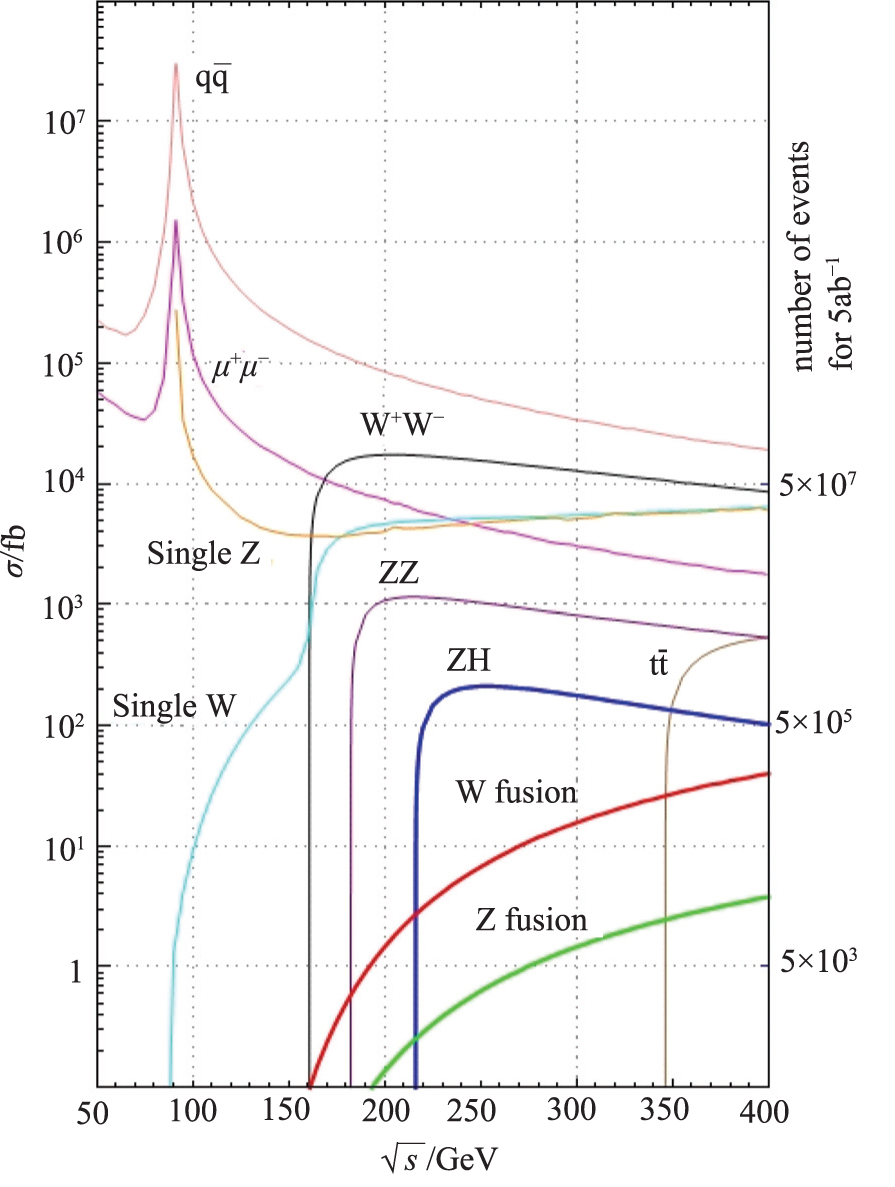
\includegraphics[width=0.98\textwidth]{Figures/ILC_cross_section.png}
\caption{\positron \electron cross section~\cite{ILC_cross}}
\end{subfigure}
\begin{subfigure}[b]{0.4\textwidth}
\includegraphics[width=\textwidth]{Figures/LHC_cross_section.png}
\caption{pp cross section~\cite{LHC_cross}}
\end{subfigure}
\caption[Cross sections for ILC and LHC]{Cross section at \positron \electron and pp colliders as a function of the collision energy. }%https://arxiv.org/pdf/hep-ph/0410364.pdf
\label{fig:Cross_sections}
\end{figure}

\section{Backgrounds}
\label{Backgrounds}
As discussed in the section above, there are no QCD processes at lepton colliders.
Instead, the beam particles are elementary and their energies are well defined, which has a big impact not only on the possible physics processes but also on the background sources for the particle detectors.
At hadron colliders, the backgrounds are dominated by the QCD background and by underlying events, since the actual collision happens between constituents of the two colliding hadrons.
The remaining constituents, however, do not disappear but hadronize and leave their traces in the detector as well.
Since this is not the case in lepton collisions, the events are in comparison very clean.
Nonetheless, there are still different background sources, from beam-beam interactions and from interactions of the beam particles with the accelerator itself.
The background processes will now be explained in detail in the following.

\subsection{High cross section backgrounds from beam-beam interactions}
\label{BeamBeam}
A significant background source for the particle detectors arises from the electromagnetic fields created by the highly focused beam bunches.
Before collision, the particle beams are focused down to a small beam size, which enhances the electromagnetic field around the bunches.
This causes the beam particles to emit photons in the forward direction, the so-called beamstrahlung.
\todo{I just counted, you say so-called 48 times in your thesis so far}
\\For a lepton beam with N beam particles per bunch and with the beam dimensions $\sigma_{x,y,z}$, one can calculate the average energy $E_{\gamma}$ of the beamstrahlung photons~\cite{Beamstrahlung_CLIC}: \todo{Check page number}
\begin{equation}
 E_{\gamma} \propto \frac{N}{(\sigma_x+\sigma_y)\sigma_z}
 \label{eq:pair_energy}
\end{equation}
The average number $n_{\gamma}$ of beamstrahlung photons that are emitted is proportional to:
\begin{equation}
 n_{\gamma} \propto \frac{N}{(\sigma_x+\sigma_y)}
 \label{eq:pair_number}
\end{equation}
The number of photons is therefore dependent on the beam size and the number of particles per beam bunch.
%Therefore, in ILC chapter about beam parameters: Hence flat beams with $\sigma_x\gg\sigma_y$ are used. The product of the horizontal and vertical beam sizes is small leading to high luminosity while the sum of them is large, reducing the beamstrahlung effect.
\\Beamstrahlung represents the main background source at lepton colliders.
However, it also causes the creation of other particle types that can be misinterpreted in the detectors as part of the signal events.

\subsubsection{Pair background}
\label{BeamBeam:pairs}
Due to the high density of beamstrahlung photons at the collision point, particle interactions between photons from opposite beam bunches or between photons and the actual beam particles can occur, which is illustrated in Figure~\ref{fig:Pair_production}.
Such interactions are then called beam-beam interactions, since they arise from interactions between the two colliding beams.
\begin{figure}
\centering
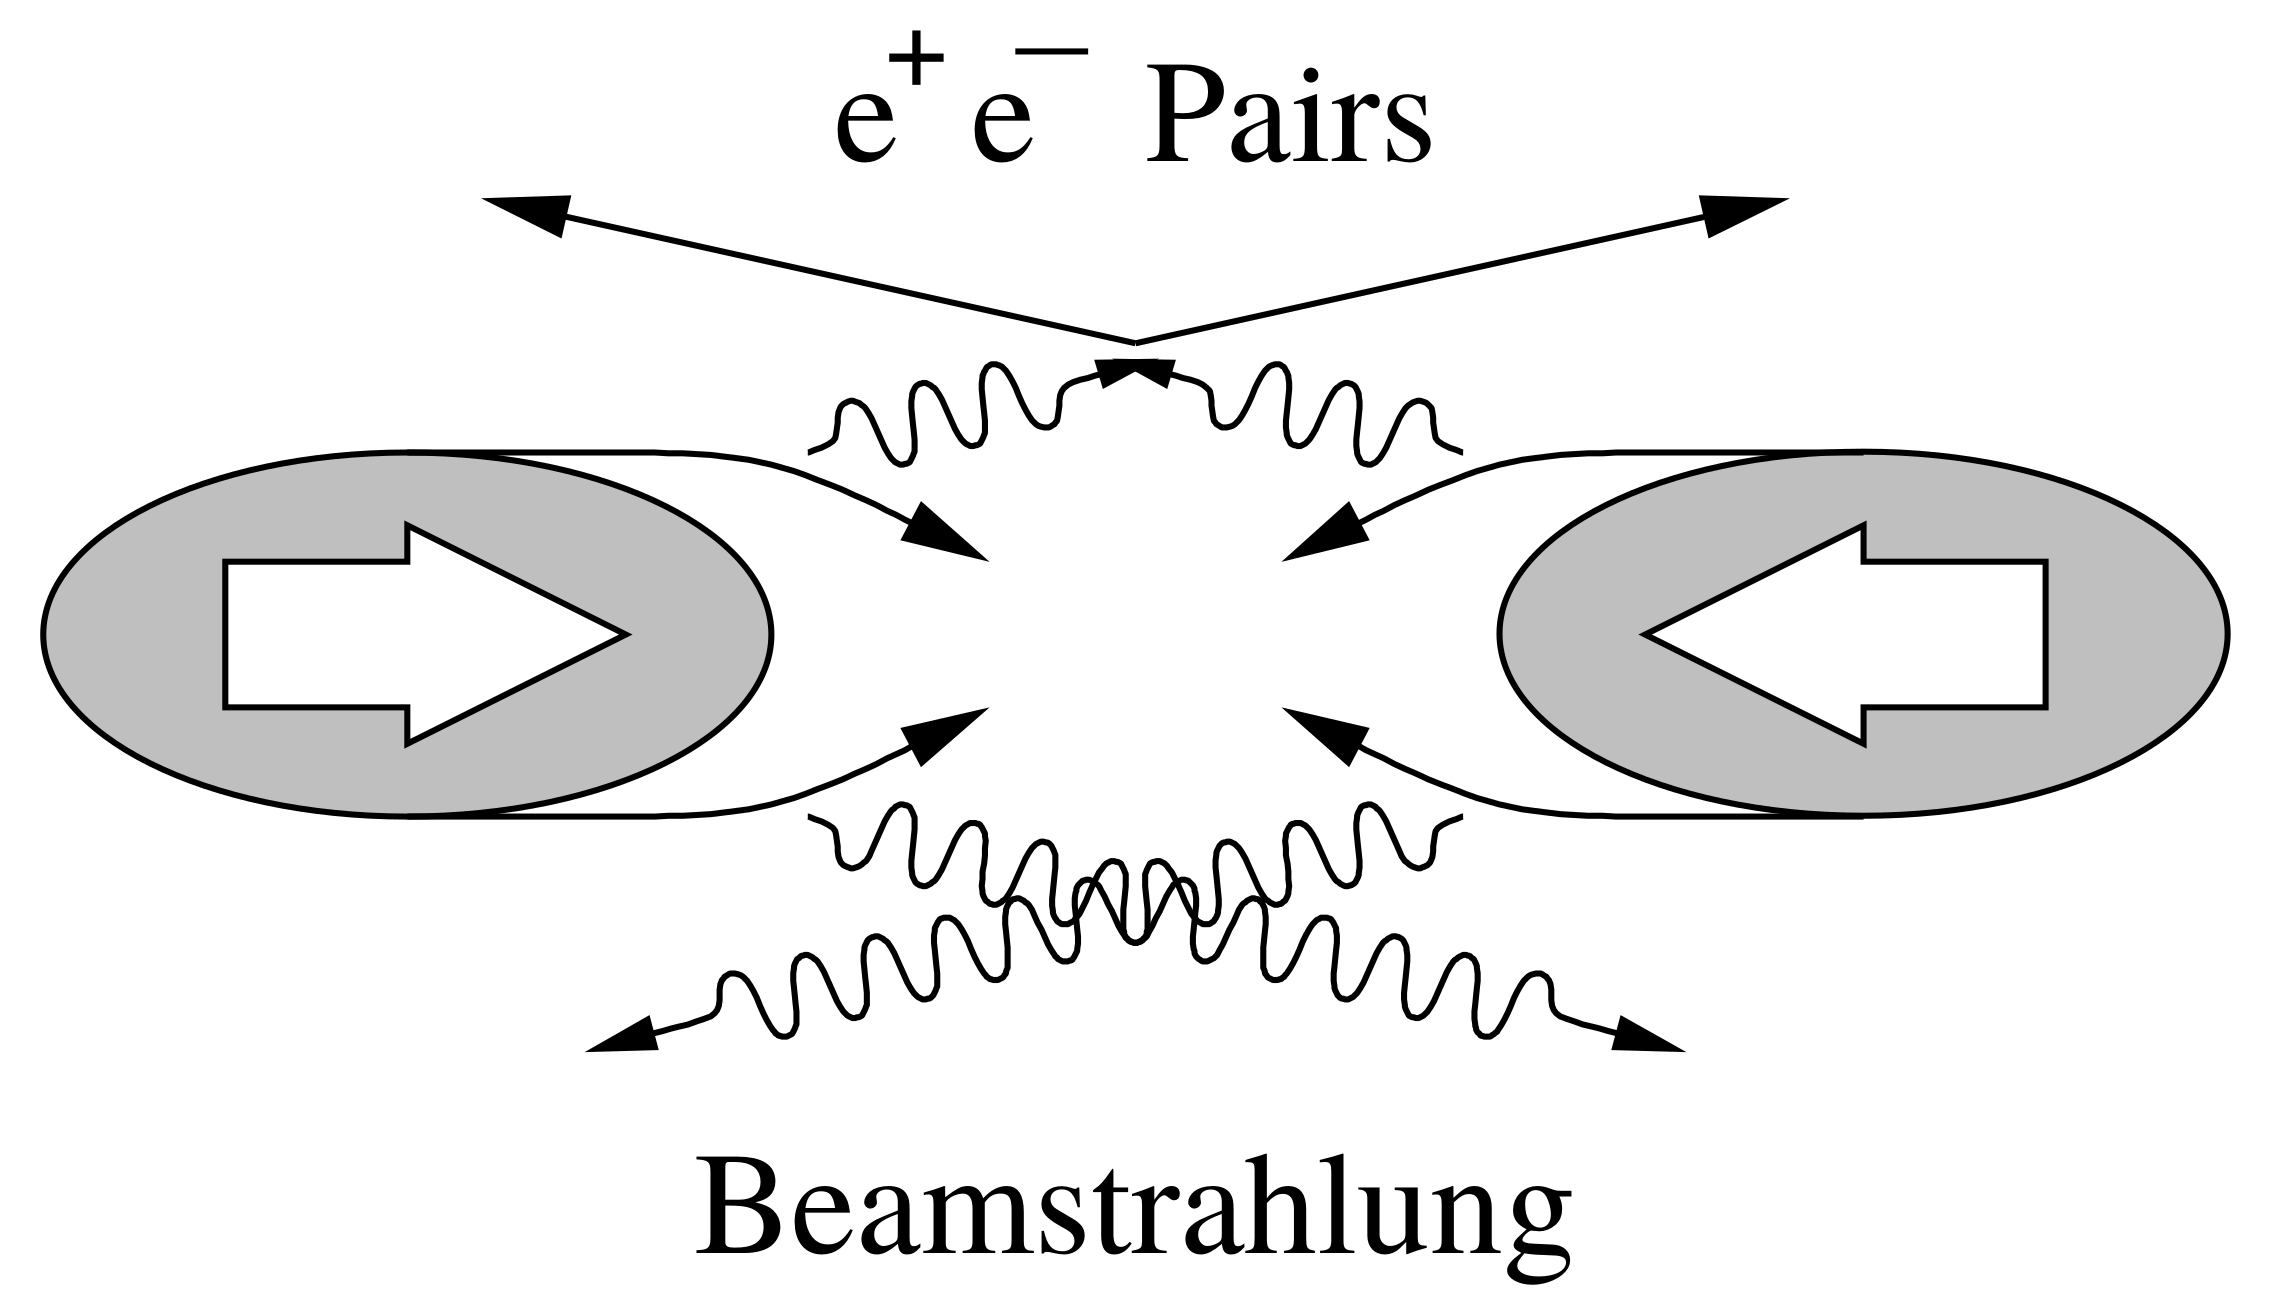
\includegraphics[width=0.4\textwidth]{Figures/PairBackground.png}
\caption{Creation of a secondary $e^+e^-$ pair through the collision of beamstrahlung photons arising from the electromagnetic field of the colliding beam bunches~\cite[]{Vogel}.}
\label{fig:Pair_production} 
\end{figure}
\\One possible outcome is the production of an electron-positron pair through three different physics processes, which are depicted in Figure~\ref{fig:Feynman:pair_production}.
In all three cases a ``secondary'' $e^+e^-$ pair is produced, either through the interaction between a beamstrahlung photon and a virtual photon emitted by a primary beam particle (Figure~\ref{fig:Feynman:pair_production} (a)),
or through the interaction of two beamstrahlung photons (Figure~\ref{fig:Feynman:pair_production} (b)),
or lastly through the interaction of two virtual photons being emitted from particles of the two opposite beams (Figure~\ref{fig:Feynman:pair_production} (c)).
\begin{figure}[h]
\begin{subfigure}[b]{0.33\textwidth}
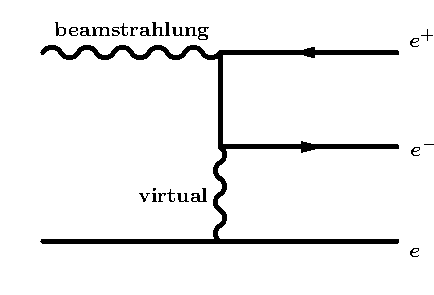
\includegraphics[width=\textwidth]{Figures/Bethe-Heitler.pdf}
\caption{Bethe-Heitler}
\end{subfigure}
\begin{subfigure}[b]{0.33\textwidth}
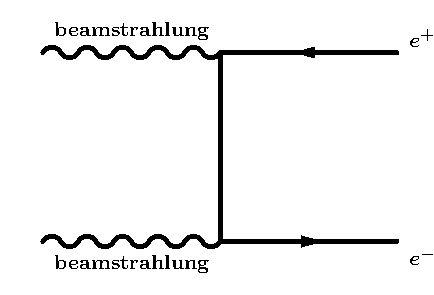
\includegraphics[width=\textwidth]{Figures/Breit-Wheeler.pdf}
\caption{Breit-Wheeler}
\end{subfigure}
\begin{subfigure}[b]{0.33\textwidth}
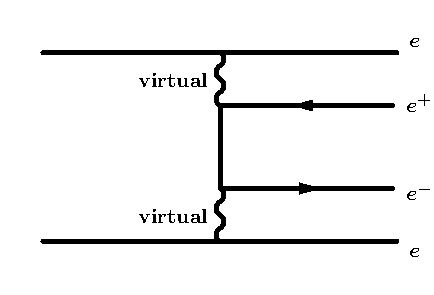
\includegraphics[width=\textwidth]{Figures/Landau-Lifshitz.pdf}
\caption{Landau-Lifschitz}
\end{subfigure}
\caption[Feynman diagrams of the production of the background pairs.]{The first-order Feynman diagrams of the production processes of background pairs at an $e^+e^-$ collider: Bethe-Heitler, Breit-Wheeler and Landau-Lifschitz.}
\label{fig:Feynman:pair_production}
\end{figure}

The produced $e^+e^-$ pairs are low $p_T$ particles, which means that they have a small momentum in the transverse beam direction.
The reason for that is the fact that the beamstrahlung photons are already boosted in the forward direction, i.e. in the beam direction.
The momentum of the secondary electrons and positrons also has a large contribution in the forward direction, and only small contributions in the transverse plane.
Further characterizations can be found in Chapter~\ref{PairBkg} about the Monte Carlo simulation of this so-called pair background.

\subsubsection{Bhabha scattering and $\gamma\gamma\rightarrow$ hadrons}
\label{BeamBeam:bhabha_gammagamma}
Further background particles are produced by processes with much smaller cross sections than for the pair background in the section above.
At the International Linear Collider for example, about 1-\num{2e5} electrons and positrons from the pair background are expected per bunch collision, whilst only around one event per bunch collision is expected for the productions of hadrons from beamstrahlung photons, and even less than one for the so-called Bhabha scattering~\cite{SiDBkgNote}. \todo{Update these numbers for 250GeV}
Figure~\ref{fig:Feynman:bhabha_gammagamma} shows the Feynman diagrams for Bhabha scattering and the $\gamma\gamma\rightarrow$ hadrons process.
Although both of these processes produce particles with low transverse momentum as well, the interaction products leave traces in the detectors, which overlay with signal physics events.
\begin{figure}[h!]
\centering
\begin{subfigure}[b]{0.35\textwidth}
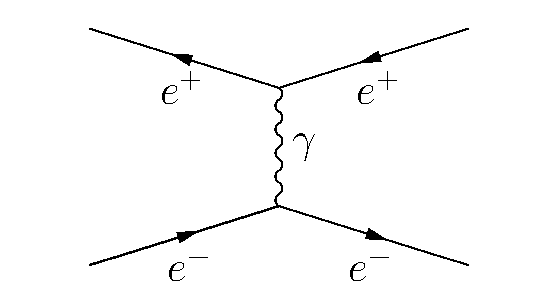
\includegraphics[width=\textwidth]{Figures/bhabha_scattering.pdf}
\caption{Bhabha scattering}
\end{subfigure}
\vspace*{0.2cm}
\begin{subfigure}[b]{0.35\textwidth}
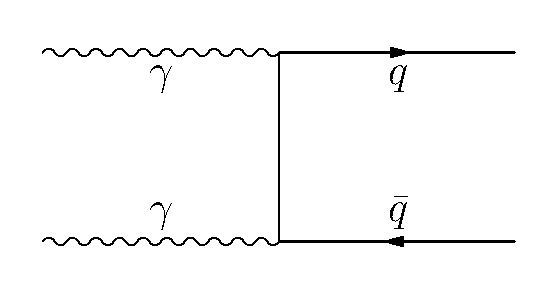
\includegraphics[width=\textwidth]{Figures/gammagamma_hadrons.pdf}
\caption{$\gamma\gamma\rightarrow$hadrons}
\end{subfigure}
\caption[Feynman diagrams of Bhabha scattering and the $\gamma\gamma\rightarrow$hadrons process.]{The first order Feynman diagrams of the Bhabha scattering and the $\gamma\gamma\rightarrow$hadrons process.}
\label{fig:Feynman:bhabha_gammagamma}
\end{figure}

\subsection{Machine backgrounds}
\label{MachineBackgrounds}

Next to the backgrounds induced from beam-beam interactions, there are also secondary particles which are created from beam interactions with the accelerator machine.
Especially those created in the proximity to the collision region can reach the particle detectors, and cause background levels that need to be investigated.
Besides synchrotron radiation photons, which are emitted by the deflection of charged particle beams in a magnetic field (see also Section~\ref{AccPhysics:Linear-Circular}), and the beamstrahlung mentioned above, the most prominent machine backgrounds are the following:
\begin{itemize}
 \item Muons emitted from beam interactions with the accelerator machine components:
 \\Due to beam orbit disruptions, the beam halo particles of the beam bunches hit components of the accelerator machine, and interact with the material.
 This leads to the emission of secondary particles, such as muons, which are boosted in the beam direction.
 When these muons are created in the final accelerator sub-systems close to the collision region, the muons reach the particle detectors and penetrate them almost perfectly horizontally due to their momentum.
 \item After the beam collision, the spent beams are passed to the beam dumps:
 \\By dumping the beam into the beam dumps, which often consist of water tanks, low momentum neutrons are produced which are directed backwards towards the collision region.
 This causes a high-radiation environment in the beam dump hall, which limits the possible duration of stay for maintenance personnel.
 On the other hand, those neutrons reaching the detectors, do not only leave tracks in the detector, but also cause radiation damage to the detector material.
\end{itemize}
All these background sources combined represent a significant background for particle detectors, and define their performance requirements.
Detailed simulations of the sources and the effect of the background particles on the detector performance is a crucial task for the research and development phase for detectors and machines, and are therefore a focus of this thesis.
Further details of the background creation and characterization are given in the respective chapters.
